\documentclass{article}
\usepackage[utf8]{inputenc}
\usepackage[russian]{babel}
\usepackage{graphicx}
\usepackage{amsmath}
\usepackage{breqn}
\usepackage{wrapfig}
\usepackage{float}
\usepackage{multirow}
\usepackage{caption}
\usepackage{subcaption}

\graphicspath{ {./data/images} }
\author{Александр Романов Б01-107}
\date{}
\title{3.3.4 Эффект Холла в проводниках}

\begin{document}
\maketitle
\section{Введение}
\subsection{Цель работы}
Измерение подвижности и конуентрации носителей заряда в проводниках.
\subsection{В работе используются} 
Электромагнит с регулируемым источником питания; вольтетр; амперметр; миллиамперметр;
милливебберметр; источник питания (1.5 V); Образец легированного германия.

\section {Работа}
\subsection{Подготовка приборов}

Проверим, что ток через образец не превышает 1 mA.

Измерим калибровочную кривую электромагнита (Учитывая параметр милливебберметра \( S\cdot N = 72 cm^2 \)): 

\begin{table}[H]
    \centering
    \begin{tabular}{|c|c|}
        \hline
        I, A  & B, T  \\\hline
        0.27  & 0.21  \\\hline
        0.54  & 0.42  \\\hline
        0.81  & 0.625 \\\hline
        1.08  & 0.79  \\\hline
        1.35  & 0.94  \\\hline
        1.62  & 1.04  \\\hline
        1.89  & 1.125 \\\hline
        2.13  & 1.16  \\\hline  
    \end{tabular}
\end{table}

\begin{figure} [H]
    \centering
    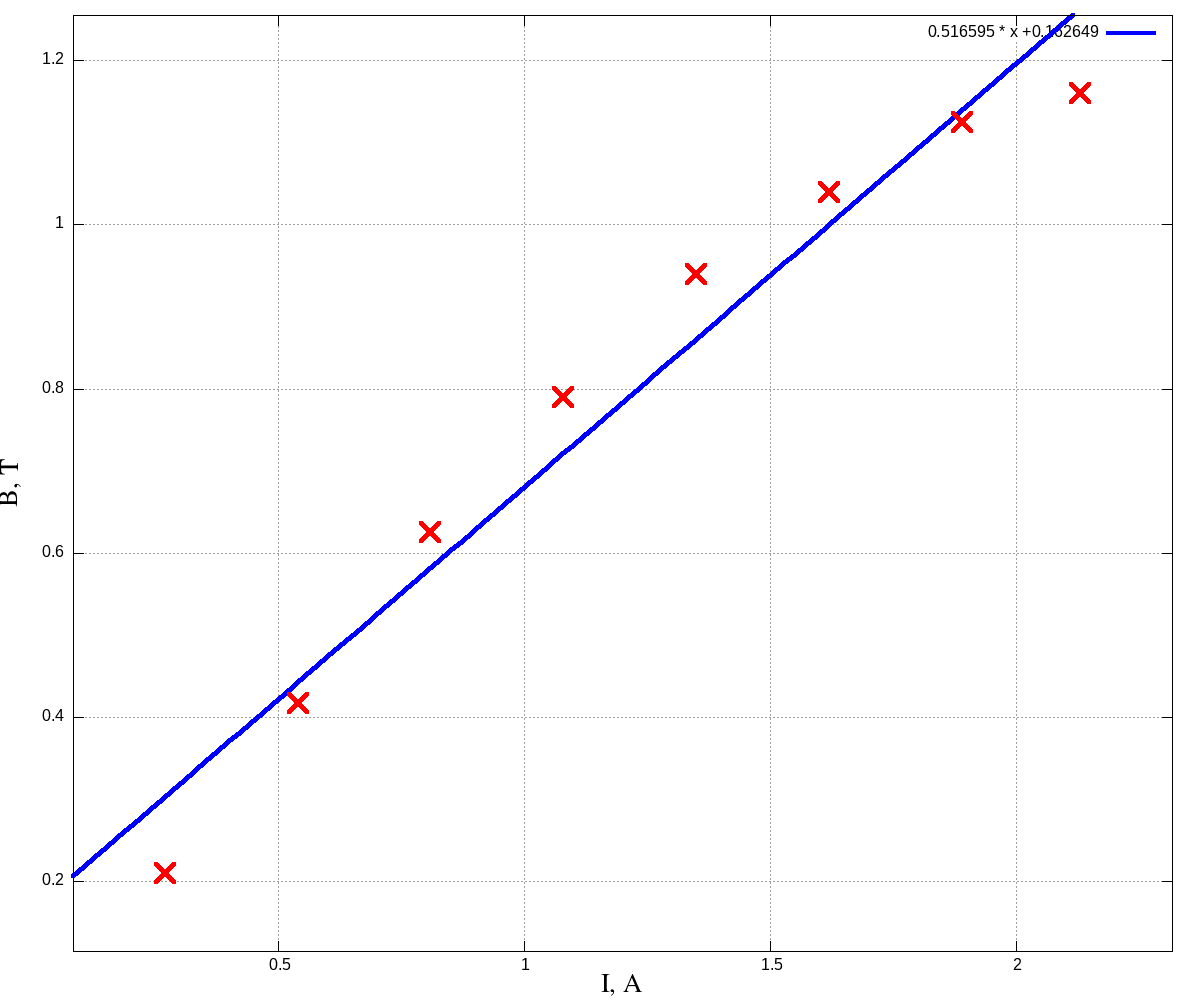
\includegraphics[width=\textwidth]{calibr_line.png}
\end{figure}

Получим зависимость:

\[ B = k\cdot I + b \]
\[ k  = (0.52 \pm 0.04) T/A \]
\[ b = (0.16 \pm 0.02) T \]

Вставим образец в зазор выключенного электромагнита и определим напряжение (\( U_0 = -0.017 \) V) между
Холловскими кантактами при минимальном точке через образец (\( I = 0.3 \) mA). Примем это значение за начало
отсчёта напряжения.

\subsection{Измерения ЭДС Холла}

Снимем зависимость холловского напряжения \(U_{34}\) от тока электромагнита \(I_{M}\) для разных токов \(I\)
через образец:

\begin{figure}[H]
    \centering
    \begin{subfigure}{.5\textwidth}
    \centering
    \begin{tabular}{|c|c|c|c|}
        \hline
        I, mA & U0, mV & Iм, A & U34, mV \\\hline
        & & 0.27 & -0.04  \\
        & & 0.54 & -0.065 \\
        & & 0.81 & -0.089 \\
        & & 1.08 & -0.111 \\
        & & 1.35 & -0.130 \\
        & & 1.62 & -0.140 \\
        & & 1.89 & -0.150 \\
        \multirow{-8}{*}{0.3}         & \multirow{-8}{*}{-0.017}       & 2.11 & -0.155 \\\hline
        & & 0.27 & 0.013  \\
        & & 0.54 & 0.044  \\
        & & 0.81 & 0.074  \\
        & & 1.08 & 0.102  \\
        & & 1.35 & 0.123  \\
        & & 1.62 & 0.138  \\
        & & 1.89 & 0.148  \\
        \multirow{-8}{*}{0.4}         & \multirow{-8}{*}{-0.017}       & 2.08 & 0.153  \\\hline
        & & 0.27 & 0.013  \\
        & & 0.54 & 0.052  \\
        & & 0.81 & 0.094  \\
        & & 1.08 & 0.127  \\
        & & 1.35 & 0.152  \\
        & & 1.62 & 0.170  \\
        & & 1.89 & 0.183  \\
        \multirow{-8}{*}{0.5} & \multirow{-8}{*}{-0.025}       & 2.07 & 0.190  \\\hline
        & & 0.27 & 0.016  \\
        & & 0.54 & 0.064  \\
        & & 0.81 & 0.110  \\
        & & 1.08 & 0.151  \\
        & & 1.35 & 0.184  \\
        & & 1.62 & 0.205  \\
        & & 1.89 & 0.220  \\
        \multirow{-8}{*}{0.6}         & \multirow{-8}{*}{-0.03}        & 2.06 & 0.228  \\\hline
    \end {tabular}
    \end{subfigure}%
    \begin{subfigure}{.5\textwidth}
        \centering
    \begin{tabular}{|c|c|c|c|}
        \hline
        I, mA & U0, mV & Iм, A & U34, mV \\\hline
        & & 0.27 & 0.017  \\
        & & 0.54 & 0.074  \\
        & & 0.81 & 0.128  \\
        & & 1.08 & 0.175  \\
        & & 1.35 & 0.214  \\
        & & 1.62 & 0.240  \\
        & & 1.89 & 0.257  \\
        \multirow{-8}{*}{0.7}         & \multirow{-8}{*}{-0.037}       & 2.04 & 0.265  \\\hline
        & & 0.27 & 0.019  \\ 
        & & 0.54 & 0.086  \\ 
        & & 0.81 & 0.145  \\ 
        & & 1.08 & 0.203  \\ 
        & & 1.35 & 0.240  \\ 
        & & 1.62 & 0.270  \\ 
        & & 1.89 & 0.292  \\ 
        \multirow{-8}{*}{0.8}         & \multirow{-8}{*}{-0.042}       & 2.04 & 0.3    \\\hline
        & & 0.27 & 0.022  \\ 
        & & 0.54 & 0.096  \\ 
        & & 0.81 & 0.165  \\ 
        & & 1.08 & 0.222  \\ 
        & & 1.35 & 0.275  \\ 
        & & 1.62 & 0.306  \\ 
        & & 1.89 & 0.328  \\ 
        \multirow{-8}{*}{0.9}         & \multirow{-8}{*}{-0.05}        & 2.03 & 0.339  \\\hline
        & & 0.27 & 0.027  \\ 
        & & 0.54 & 0.103  \\ 
        & & 0.81 & 0.180  \\ 
        & & 1.08 & 0.250  \\ 
        & & 1.35 & 0.302  \\ 
        & & 1.62 & 0.340  \\ 
        & & 1.89 & 0.365  \\ 
        \multirow{-8}{*}{1}           & \multirow{-8}{*}{-0.055}       & 2.03 & 0.375 \\\hline
        \end{tabular}
    \end{subfigure}%
\end{figure}

Изобразим все графики \(U(B)\) на одном чертеже:

\begin{figure}[H]
    \centering
    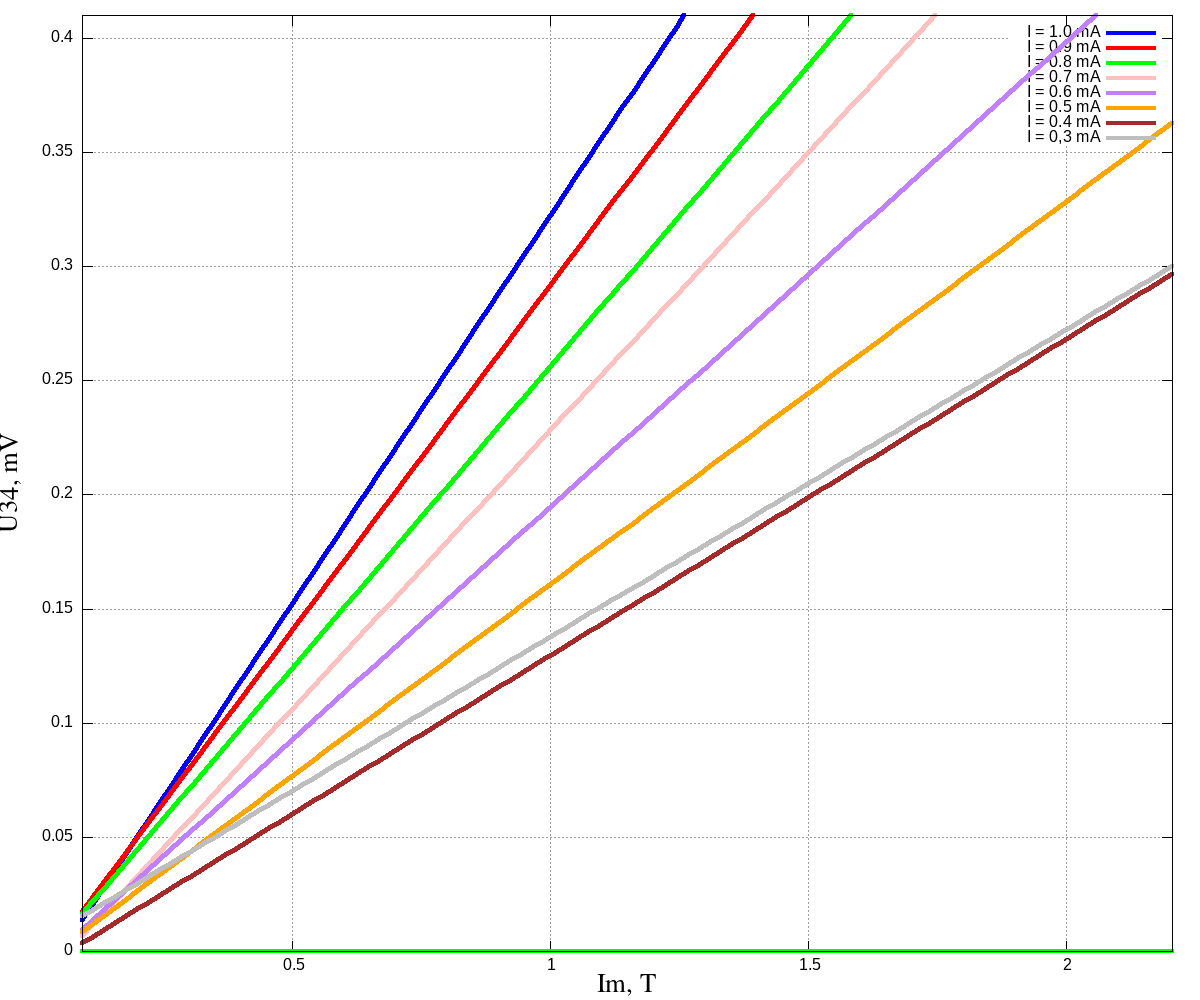
\includegraphics[width=\textwidth]{multy-plot.png}
\end{figure}
    

Угловые коэффициенты полученных прямых \( U = k \cdot B + b \):

\begin{table}[H]
    \centering
    \begin{tabular}{|c|c|}
        \hline
        \( I, mA \) & \( k, mV/T \)\\\hline
        0.3 & \( 0.135 \pm 0.006 \) \\\hline
        0.4 & \( 0.139 \pm 0.007 \) \\\hline
        0.5 & \( 0.168 \pm 0.008 \) \\\hline
        0.6 & \( 0.204 \pm 0.01  \) \\\hline
        0.7 & \( 0.244 \pm 0.01  \) \\\hline
        0.8 & \( 0.264 \pm 0.007 \) \\\hline
        0.9 & \( 0.302 \pm 0.011 \) \\\hline
        1.0 & \( 0.340 \pm 0.015 \) \\\hline
    \end{tabular}
\end{table}

Построим график \( k(B) \):

\begin{figure}[H]
    \centering
    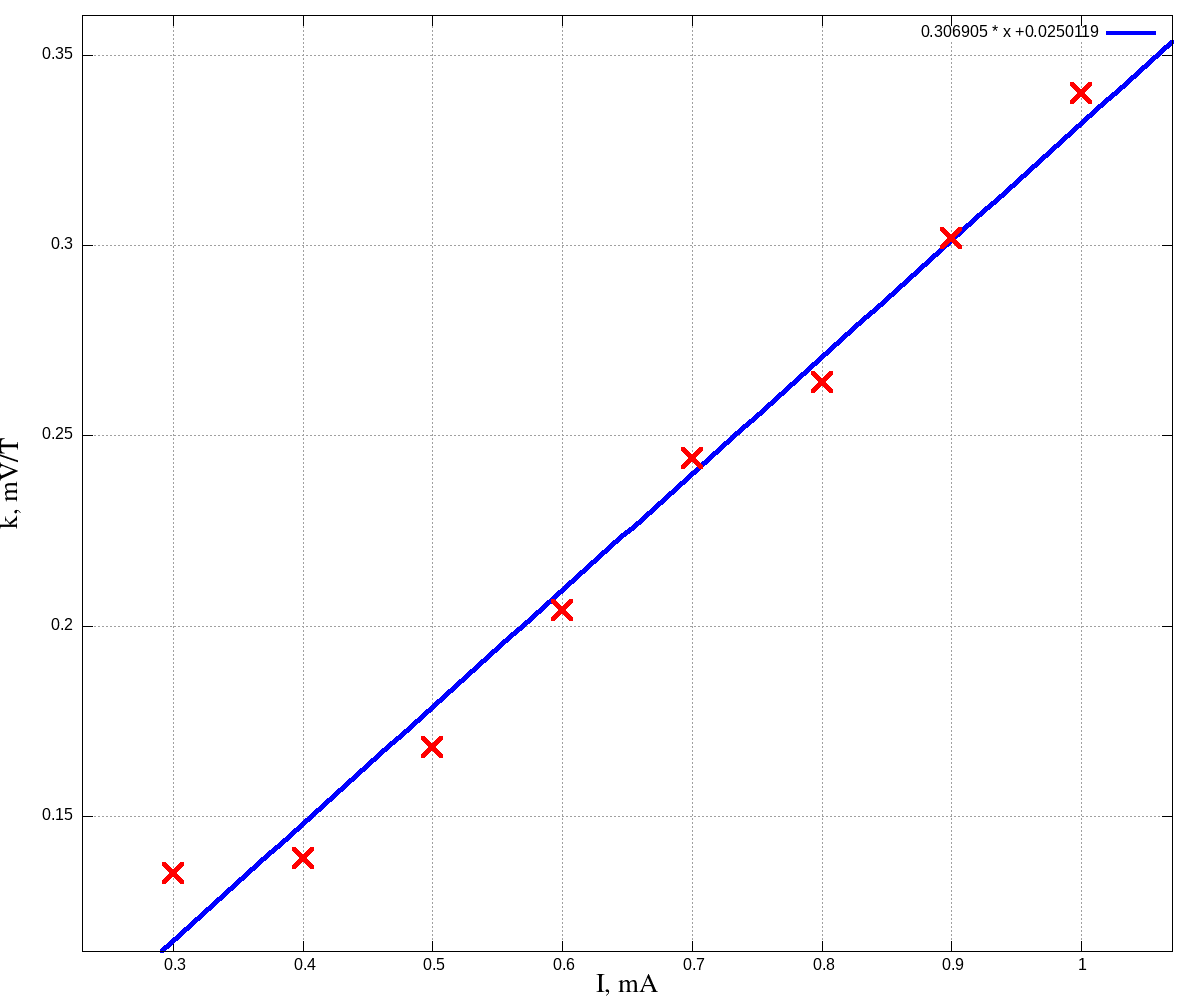
\includegraphics[width=\textwidth]{k-I.png}
\end{figure}

Получилась зависимость \( k = a \cdot I + b \), где
\[ a = (0.31 \pm 0.014)\; \frac{V}{T\cdot A} \]
\[ b = (0.025 \pm 0.003)\; mV/T \]

Отсюда по формуле:
\[ a = \frac{U34}{B\cdot I} = \frac{R_H}{h} \]
Можно вычислить величину постоянной Холла (Учитывая \(h = 1.5 mm\)):
\[ R_H = a\cdot h = (0.47 \pm 0.02) \; 10^{-3}\frac{V\cdot m}{T\cdot A} \]

Тогда отсюда согласно формуле
\[ R_H = \frac{1}{n\cdot e} \]
Получим значение концентрации \(n\) свободных носителей заряда в образце:
\[ n = (1.33 \pm 0.31)\; 10^{-22}m^{-3} \]

Расчитаем теперь Удельную проводимость образца. По формуле:
\[ \sigma = \frac{I\cdot L_{35}}{U_{35}al} \]
Взяв измеренные значения (\( I = 1.0\; mA, U_{35} = 1.681\; mV \))и учтя параметры
образца (\(L_{35} = 3.0\; mm, h = 1.5\; mm, l = 1.7\; mm\)) получим:

\[ \sigma = (699.8 \pm 81)\; (\Omega\cdot m) \]

Расчиатем подвижность носителей заряда по формуле:
\[ b = \frac{\sigma}{en} = \sigma\cdot R_H = (3285 \pm 395)\; \frac{cm^2}{V\cdot s} \]

\section{Выводы}

\end{document}